\documentclass{nle}

\usepackage{booktabs} % For formal tables
\usepackage[utf8]{inputenc}
\usepackage{graphicx}
\usepackage{mathtools}
\usepackage{amsfonts}
\usepackage{multirow}
\usepackage{glossaries}
\usepackage{tikz}
\usepackage{pgfplots}

\DeclareMathOperator*{\argmax}{arg\,max\,}
\renewcommand{\arraystretch}{1.2}

\makeglossaries
\newacronym{nlp}{NLP}{Natural Language Processing}
\newacronym{wde}{WDE}{Web Data Extraction}
\newacronym{ner}{NER}{Named Entity Recognition}
\newacronym{hmm}{HMM}{Hidden Markov Models}
\newacronym{crf}{CRF}{Conditional Random Fields}
\newacronym{lstm}{LSTM}{Long Short-Term Memory Networks}
\newacronym{ie}{IE}{Information Extraction}
\newacronym{rne}{RNE}{Researcher Name Extraction}
\newacronym{rnn}{RNN}{Recurrent Neural Networks}
\newacronym{cnn}{CNN}{Convolutional Neural Networks}
\newacronym{pos}{POS}{Part-of-Speech}

\begin{document}

\title{Named Entity Recognition for Web Data Extraction}

\author[João Mateus de Freitas Veneroso and Berthier Ribeiro-Neto]
       {João Mateus de Freitas Veneroso$^A$ \and
        Berthier Ribeiro-Neto$^B$\\
	Universidade Federal de Minas Gerais$^{A,B}$ \\
	Google Engineering$^B$, Belo Horizonte - MG, Brazil}

% \affiliation{%
%   \institution{Universidade Federal de Minas Gerais}
%   \streetaddress{Av. Pres. Antônio Carlos, 6627 - Pampulha}
%   \city{Belo Horizonte}
%   \state{MG}
%   \postcode{31270-901}
%   \country{Brazil}}
% \email{jmfveneroso@gmail.com}
% 
% \author{Berthier Ribeiro-Neto}
% \affiliation{%
%   \institution{Universidade Federal de Minas Gerais}
%   \streetaddress{Av. Pres. Antônio Carlos, 6627 - Pampulha}
%   \city{Belo Horizonte}
%   \state{MG}
%   \postcode{31270-901}
%   \country{Brazil}}
% \email{berthier@dcc.ufmg.br}
% \email{berthier@google.com}

\maketitle

\begin{abstract}

% \gls{wde} methods often rely on hand-coded rules to 
% identify and extract data from webpages. These methods are usually
% suited for extracting information from pages within
% the same website, however they perform poorly on extraction 
% tasks across different websites. Alternatively, statistical and 
% machine-learning-based sequence labeling methods provide a more flexible 
% approach to Web data extraction. Many times, HTML pages are very different 
% from plain text, because sentences are too short to provide adequate 
% context for conventional Named Entity Recognition methods to work 
% properly. Also, the HTML structure may encode information that is not 
% replicated in the text. Nonetheless, these limitations can be overcome by
% adequate feature engineering, the use of pretrained word 
% embeddings and neural character representations. In this article, we 
% evaluate the performance of different methods of named entity recognition 
% on the task of Web data extraction. In particular, we introduce a novel 
% dataset\footnote{The dataset and all models discussed in this article are 
% available in: https://github.com/jmfveneroso/ner-on-html.} 
% consisting of faculty listings from university webpages across
% the world in multiple languages and test the NER models on the task of 
% extracting researcher names from these listings. We found that a 
% neural network architecture that combines a bidirectional LSTM with
% a Conditional Random Fields output layer and LSTM-based character 
% representations outperforms other methods on the researcher name 
% extraction task, achieving an F1-score of 0.8867 with no feature engineering. 
% With the addition of hand crafted features, the F1-score can be slightly 
% improved to 0.8995.

Web Data Extraction methods often rely on hand-coded rules to 
identify and extract data from webpages. These methods are
suited for extracting information from pages within
the same website, however they perform poorly on extraction 
tasks across different websites. Alternatively, 
machine-learning-based Named Entity Recognition methods provide a more flexible 
approach to Web Data Extraction. However, many times webpages are very different 
from plain text, because sentences are too short to provide adequate 
context for conventional Named Entity Recognition models to work 
properly. 
% Nonetheless, the HTML structure also encodes useful information that 
% can be used by NER models to achieve a better performance. We propose a
% method to use this information: the self-training strategy for Hidden Markov
% Models.
In this article, we 
evaluate the performance of different methods of Named Entity Recognition
in the task of Web Data Extraction. In particular, we introduce a novel 
dataset consisting of faculty listings from university webpages across
the world in multiple languages and test different Named Entity Recognition 
models in the task of 
extracting researcher names from these listings. We found that a 
neural network architecture that combines a bidirectional LSTM with
a Conditional Random Fields output layer and LSTM-based character 
representations outperforms other methods achieving 90.2 F1 in 
the task. However, with the self-training strategy, we can get a much simpler 
model, the second-order Hidden Markov Model, to achieve 87.9 F1.

\end{abstract}

\section{Introduction}

\gls{wde} is the task of automatically extracting structured 
information from unstructured or semi-structured web documents. The input 
usually consists of web documents containing a number of predetermined entities 
organized in a similar manner. The \gls{wde} task consists of 
identifying these entities and organizing them according to a template. 

HTML documents most often lie in between the structured/unstructured 
data paradigm. DOM hierarchy, element disposition, CSS classes, and other 
features related to the document structure and indirectly associated with the 
data itself can be valuable information on the task of identifying
entities. Yet, we cannot expect these features to be completely constrained 
by an underlying pattern. Organization patterns tend to follow some guidelines 
but they are in no way subject to strict rules. That is why classical \gls{wde} 
systems such as automatic wrapper generators 
\cite{Kushmerick2000,Hsu1998,Muslea1999}
do not translate very well across different websites. 

Most existing \gls{wde} methods are tailored to extract data 
from a single webpage, producing different compromises between efficacy and 
degree of human supervision. Some unsupervised approaches proposed to tackle 
the problem of data extraction for whole application domains 
\cite{Crescenzi2001}. Usually, 
unsupervised \gls{wde} methods work in two stages. In the record segmentation stage,
WDE systems seek to cluster visually and structurally similar webpage regions 
and identify repeating data records with heuristics and 
hand-coded rules. In the attribute labeling stage, WDE systems seek to identify 
the correct attributes on data records, many times resorting to regular expressions 
or gazetteer matching strategies. The outcome of each of these stages can aid one 
another. The inner patterns of data records can help in identifying attributes of other 
data records. Also, by properly identifying data record attributes, it becomes 
easier to determine boundaries and perform record segmentation.

While unsupervised approaches can be sometimes adequate to extract information from 
webpages with similar templates, they usually fail on cross-website data extraction 
tasks. Also, more sophisticated approaches may be needed when we are not dealing
with easily distinguishable attributes such as prices and dates. 
Comparatively, statistical machine learning provides more robust and flexible methods
of \gls{wde}. In recent years, we saw amazing progress in 
the field of \gls{nlp} that is extremely relevant to
the \gls{wde} community, particularly with the introduction of Deep Neural Networks 
for Sequence Labeling~\cite{Collobert2011}, but these advancements were 
not widely incorporated by \gls{wde} systems. Also, most of the attention of the \gls{nlp} community 
regarding this topic is devoted to solving \gls{ie} tasks in plain text, such as 
the identification of people and organizations in news texts.
However, the difference between some types of webpages and plain text is significant, so
\gls{ie} systems trained in plain text datasets tend to perform poorly 
when confronted with some web extraction tasks, as we have confirmed in our experiments.

A concrete example of a \gls{wde} problem that demands the type of
flexible solution provided by statistical machine learning methods is the extraction of 
researcher names from faculty directories. Automatically extracting researcher information 
from university websites is important, for example, to construct researcher affiliation databases 
and compare the academic impact of research groups using bibliographic indices~\cite{Ribas2015}. 
The problem of \gls{rne} can be solved with machine learning methods of 
\gls{ner}.

Many \gls{wde} tasks in the web share a common
factor with the \gls{rne} task. That is, they need to extract similar
entities from different webpages or they need to extract entities from short snippets of text 
instead of complete sentences. Some examples would be comment extraction from blog
posts and \gls{ner} in tweets. Because of the lack of context in tweets, \gls{ner} methods trained 
in conventional plain text corpora tend to perform badly for more or less the same reasons 
they perform badly in other \gls{wde} tasks.

In this article, we compare different machine learning approaches to 
\gls{ner} on the web by evaluating their performance in the 
\gls{rne} task. With this purpose in mind, we introduce a novel \gls{ner} dataset 
with labeled entities, consisting of faculty directories from universities across the world,
the RNE dataset~\footnote{
The dataset is available in https://github.com/jmfveneroso/ner-on-html.
}.
We compare the models in terms of their Precision, Recall, F-scores and their 
overall complexity. That is, even if a model has a slightly worse performance in terms of the
objective evaluation metrics in comparison to other approaches, it may still be useful if it 
is considerably simpler and faster to train.
The tested models were the \gls{hmm} up to third order, \gls{crf}, and a range of Deep Learning 
architectures based on Bidirectional \gls{lstm}. We also 
introduce the self-training strategy that can boost the performance 
of \gls{hmm}s in sequence labeling tasks for the web. 

The usability of the evaluated models is not limited to the particular problem of \gls{rne}. 
By reliably detecting named entities on the web, we can boost the performance 
of existing \gls{wde} approaches or even construct an end-to-end architecture that
solves the problem of data extraction across different websites with improved robustness. Also, 
the researcher affiliation database constructed with the application of these methods will
be made public in the future to provide deeper insight in bibliometric studies about the
scientific impact of research groups.


\section{Related Work}
\label{cha:related_work}

The \gls{rne} task is a problem in \gls{wde} that
we proposed to solve with the application of machine learning methods of \gls{ner}.
This section presents the related research in the fields of \gls{wde} 
in Section~\ref{sec:wde} and \gls{ner} in Section~\ref{sec:ner}.

\subsection{Web Data Extraction}
\label{sec:wde}

Since the early 1990s, the astonishing growth of public information in the web has 
led to the development of a number of different approaches to the problem of \gls{wde}.
Traditionally, the task was solved by designing special purpose
programs called wrappers to recognize relevant data and store records in a structured
format. These early tools varied wildly relative to their degree of automation. 

It was readily perceived that manual wrapper generation was a rather tedious and
error prone process, unsuited for large scale operations. Wrappers tend to
break frequently because they rely on webpage features that can change 
often. So, in the late nineties, several authors advocated for wrapper induction, a technique 
that consists of automatically constructing wrappers from a small set of examples by 
identifying delimiters or context tokens that single out the desired attributes. 
Some remarkable wrapper induction methods are WIEN~\cite{Kushmerick2000}, Soft 
Mealy~\cite{Hsu1998} and STALKER~\cite{Muslea1999}.

Despite being better than constructing wrappers manually, wrapper induction methods 
still suffered from a lack of expressive power and flexibility. These methods had 
trouble handling records with missing attributes or unusual structures because
patterns could only be identified if they happened at least once in the examples.

Other approaches such as NoDoSE~\cite{Adelberg1998} and Debye~\cite{Laender2002a} 
brought greater flexibility to wrapper induction methods by requiring a greater level 
of human interaction through graphical user interfaces. \gls{wde} techniques often 
require some sort of assistance from human experts to boost accuracy. One of the main challenges 
in the field lies in determining an adequate trade-off between the degree of automation and 
the Precision and Recall of the data extraction tool.

To automate the task of \gls{wde} completely some approaches,
such as Road Runner~\cite{Crescenzi2001}, removed entirely the need for data examples.
Road Runner parses documents belonging to a same class (e.g. books in Amazon) and 
generates wrappers based on their similarities and differences, yielding comparable results 
to those obtained by wrapper induction methods. However, like previous approaches, it was 
unsuited for cross site extraction tasks because the learned rules were not general enough.

Early NLP-based approaches aimed at extracting more general rules that could possibly
be employed over multiple websites. RAPIER~\cite{Califf1999} is a method of rule
extraction that uses information such as part-of-speech tags and semantic classes from
a lexicon to derive patterns from a set of training examples. This approach is more
flexible than the wrapper induction methods, however it achieves much lower rates of 
Precision and Recall.

A survey by Laender, Ribeiro-Neto, da Silva and Teixeira~\shortcite{Laender2002b} made a thorough classification of the
early approaches with a taxonomy based on their main technology, being them: languages for
wrapper development, HTML-aware tools, NLP-based tools, Wrapper Induction Tools,
Modeling-based tools and Ontology-based tools. Some noteworthy examples from this era
are: 
%
\begin{itemize}
\item TSIMMIS~\cite{Hammer1997} and WebOQL~\cite{Arocena1999}, which are special purpose 
languages for building wrappers.
\item Road Runner~\cite{Crescenzi2001}, XWRAP~\cite{Liu2000} and W4F~\cite{Sahuguet1999}, 
which are HTML-aware tools that infer meaningful patterns from the HTML structure.
\item RAPIER~\cite{Califf1999}, SRV~\cite{Freitag1998}, WHISK~\cite{Soderland1999}, which 
are NLP-based tools.
\item WIEN~\cite{Kushmerick2000}, Soft Mealy~\cite{Hsu1998} and STALKER~\cite{Muslea1999} which 
are wrapper induction methods.
\item NoDoSE~\cite{Adelberg1998} and Debye~\cite{Laender2002a}, which are semi-supervised
tools that require some interaction with the user by means of a graphical
user interface.
\end{itemize}
%
% Text Runner.
% https://www.aaai.org/Papers/IJCAI/2007/IJCAI07-429.pdf
\cite{Chang2006} complemented the previous surveys with semi-supervised 
technologies such as Thresher~\cite{Hogue2005}, IEPAD~\cite{Chang2001} and 
OLERA~\cite{Chang2004}. They differed from supervised 
and unsupervised methods because they either needed only a rough description of
data from users for extraction rule generation or some level of post processing
that needed user attention. 
%The survey also mentioned newer unsupervised methods
% such as DeLa~\cite{Wang2003}, Exalg~\cite{Arasu2003} and Depta~\cite{Zhai2005}.

Most of the early \gls{wde} systems were rule-based with either 
manual rule description or automatic rule learning from examples, thus they
suffered from a lack of flexibility when dealing with noisy and unstructured data.
Huge progress in the field of statistical learning led to the development of
models that tried to solve this problem.

Sarawagi~\shortcite{Sarawagi2008} introduced a classification that segmented wrappers in
rule-based methods, statistical methods and hybrid models, bringing together 
the fields of \gls{ner}, Relationship Extraction and \gls{wde}. 
The rule based methods encompass most of the previous models. While the statistical methods 
convert the extraction task into a token labeling task, solved with \gls{ner} 
and Relationship Extractions methods. Traditionally, these subtasks were solved with 
generative models based on \gls{hmm}s or discriminative models based on the 
Maximum Entropy principle, but recently these have been largely superseded by Deep Neural 
Networks. Different from automatic wrapper generators, statistical methods are suitable for
a large variety of tasks, especially when we want the system to handle cross website information 
extraction and plain text information extraction. That is why this class of methods is of 
special interest to our application. The progress of statistical models will be 
discussed in Section~\ref{sec:ner}.

Recent surveys by Ferrara, De Meo, Fiumara and Baumgartner~\shortcite{Ferrara2014}, 
Schulz, Lassig and Gaedke~\shortcite{Schulz2016} and
Varlamov and Turdakov~\shortcite{Varlamov2016}
updated the previous surveys on Information Extraction methods with some interesting innovations. 
Some examples are: the Visual Box Model~\cite{Krupl2005}, a data extraction system that produces 
a visualization of the webpage to exploit visual cues to identify records presented in a tabular form;
automatic wrapper adaptation~\cite{Ferrara2011}, a technique that tries to reduce the cost of 
wrapper maintenance by measuring the similarity of HTML trees and adapting
wrappers to the new page structure; AutoRM~\cite{Shi2015}, a method to mine
records from a single webpage by identifying similar data regions through DOM
tree analysis; and Knowledge Vault~\cite{Dong2014}, a method that combines different 
extraction approaches to feed a probabilistic knowledge base.

Most data extraction systems focus on extracting information from single websites
and are therefore unsuited for cross website extraction tasks. Even unsupervised
approaches that are application domain independent, such as RoadRunner and EXALG, 
only work well when extracting data from pages generated from a same template. 

A statistical approach to unsupervised domain 
independent \gls{wde} was described by Zhu, Nie, Wen, Zhang, and Ma~\shortcite{Zhu2005}. The 2D CRF 
model takes a webpage segmented into data blocks and employs a two dimensional \gls{crf}
model to perform attribute labeling. The model was further improved~\cite{Zhu2006} to model 
record segmentation and attribute labeling as a joint task.
Some of the limitations of early unsupervised methods 
were also addressed by ObjectRunner~\cite{Abdessalem2010} and DIADEM~\cite{Furche2012}. 
These methods work by annotating webpages automatically with regular expressions, gazetteers and 
knowledge bases. They can rectify low quality annotations and even improve the annotators
by exploring regular structures in the DOM during the record segmentation phase.

\gls{wde} methods have undoubtedly improved extraordinarily, but
as pointed by Schulz, Lassig and Gaedke~\shortcite{Schulz2016}, it is difficult to compare the results 
achieved by competing tools. Also, many tools seem to rely excessively on heuristic methods.
The recent advancements in sequence taggers may provide more robust and flexible techniques
to address this problem.


\subsection{Named Entity Recognition}
\label{sec:ner}

\gls{ner} is an important subtask in \gls{ie}.
The \gls{ner} task was defined in the Third Message 
Understanding Conference (MUC-3)~\cite{Sundheim1991}, where researchers were asked to extract
entities from a news corpus about terrorist incidents. However, it was the 
language-independent \gls{ner} shared task at the Conference 
on Computational Natural Language Learning in 2003 ({CoNLL-2003})~\cite{KimSang2003},
that established an enduring labeled dataset constructed with news texts from Reuters.
Despite its reduced size and the limited variability of its documents, the {CoNLL-2003}
dataset is still used to compare the performance of NER systems in English and 
German. 

Sequence labeling for \gls{ner} and \gls{pos} tagging (labeling nouns, verbs, pronouns, etc.) 
is very similar, so, many times, research articles that propose new methods for \gls{ner}
also report results for the \gls{pos} Tagging task. And frequently, the best methods for 
\gls{pos} Tagging are also the best methods for \gls{ner}.

Traditionally, the \gls{ner} task was solved with generative models based on 
\gls{hmm}s. The first appearance of \gls{hmm}s in the
field of \gls{nlp} occurred in the mid-seventies and was
primarily focused on the problem of Speech Recognition. 
But in the late nineties, \gls{hmm}s also found important applications in \gls{ie}
and \gls{ner} as in the works by Bikel, Schwartz and Weischedel~\shortcite{Bikel1999}, 
Freitag and Mccallum~\shortcite{Freitag1999}, 
and Freitag and Mccallum~\shortcite{Freitag2000}.

The problem with \gls{hmm}s is that they model the joint probability between 
sequences of observations and labels $ P(X, Y) $, a harder problem than modelling the corresponding 
conditional probability $ P(Y|X) $. They assume conditional independence for the observations $ X $, and
therefore, they cannot handle overlapping features. This lack of flexibility led to the 
development of discriminative approaches to sequence labeling based on the Maximum Entropy principle.

Some early examples are Maximum Entropy Taggers for NER~\cite{Borthwick1998} and
\gls{pos} Tagging~\cite{Ratnaparkhi1998}. The Maximum Entropy Markov Model~\cite{McCallum2000} 
was developed just a while later, building up on the intuition of \gls{hmm}s combined with
the flexibility of discriminative approaches. However, because of the label bias problem,
this model was superseded by \gls{crf}s~\cite{Lafferty2001}. % McCallum2003
At this time, the best performing systems almost always resorted to external gazetteers 
and hand-chosen features, as is the case for the {CoNLL-2003} winning model~\cite{Florian2003}.

With the advancement of Machine Learning in recent years, we saw the rise
of Neural Networks applied to sequence labeling. In 2011, \cite{Collobert2011} 
introduced Neural Networks free of feature engineering to sequence labeling tasks,
using \gls{cnn} over word embeddings with a CRF output layer to tackle 
the problems of \gls{pos} tagging, Chunking, Semantic Role Labeling, and NER. A similar architecture 
proposed in 2015 by~\cite{Huang2015}, the Bi-LSTM-CRF, replaced the \gls{cnn} in \cite{Collobert2011} 
with a bidirectional LSTM, achieving better results.

In 2016, further advancement to the NER models was achieved by incorporating character 
representations at the bottom of the Bi-LSTM-CRF architecture to extract morphological 
features from words automatically. The model by~\cite{Lample2016} uses a 
bidirectional \gls{lstm} over character embeddings and the model by~\cite{Ma2016} uses a
one dimensional \gls{cnn} with max pooling over character embeddings. Both models also 
made use of pre-trained GloVe word embeddings, created by~\cite{Pennington2014}.

Small improvements to NER systems have been made since then, primarily due to the 
introduction of new word embeddings on variations of the Bi-LSTM-CRF architecture. From
this group, we can mention ELMo~\cite{Peters2018}, BERT~\cite{Devlin2018}, and
Flair~\cite{Akbik2018}. 
All of them were introduced in 2018 and they differ primarily 
in how to construct contextual embeddings from the internal states of a language 
modelling neural network.

To our knowledge, the best NER system up to this date (considering the performance in the
{CoNLL-2003} dataset) is the bidirectional transformer model proposed by Baevski, Edunov, Liu, Zettlemoyer and Auli~\shortcite{Baevski2019} that uses
a stack of self-attention modules and ELMo embeddings. Table~\ref{tab:ner_model_comparison}
shows a comparison of the history of reported F1 scores in the English test set of the {CoNLL-2003} dataset
for the NER systems that were mentioned in this section. Each of the mentioned systems held the 
record for the task at a given time.


\begin{table}[h]
  \small
  \begin{center}
    \begin{tabular}{ lc }
      \toprule
      Model & Test F1 \\
      \midrule
      Florian, Ittycheriah, Jing and Zhang 2003 (CoNLL-2003 Winner)            & 88.76 \\
      Collobert, Weston, Bottou, Karlen, Kavukcuoglu, and Kuksa 2011           & 89.59 \\
      Huang, Xu and Yu 2015                                                    & 90.10 \\
      Lample, Ballesteros, Subramanian, Kawakami and Dyer 2016                 & 90.94 \\
      Ma and Hovy 2016                                                         & 91.21 \\
      Peters, Neumann, Iyyer, Gardner, Clark, Lee and Zettlemoyer 2018         & 92.22 \\
      Devlin, Chang, Lee, and Toutanova 2018                                   & 92.80 \\
      Akbik, Blythe and Vollgraf 2018                                          & 93.09 \\
      Baevski, Edunov, Liu, Zettlemoyer and Auli 2019                          & 93.50 \\
      \bottomrule
    \end{tabular}
  \end{center}
  \caption{Model performances in the {CoNLL-2003} English test set.}
  \label{tab:ner_model_comparison}
\end{table}




\section{Named Entity Recognition Models}

Many \gls{wde} systems rely on hand crafted rules or gazetteers to perform
attribute annotation. Machine learning approaches to NER can improve annotations of 
more complex entities and even perform entity detection without any feature
engineering. We explored three methods of Named Entity Recognition
in the context of a \gls{wde} task. First, we discuss two traditional 
approaches: Hidden Markov Models, and Linear Chain Conditional Random Fields. Then,
we discuss neural network architectures.

\subsection{Hidden Markov Models}

A Markov Model is a stochastic model that computes the most probable sequence of states 
given a limited set of observable states $ S = \{s_1, s_2, ..., s_n \} $.
The Hidden Markov Model (HMM) differs from the Markov Model in that it
does not observe the states directly, but rather a probabilistic function of those 
states. For example in NER, the words are observed, however the Named Entity labels
associated with these words are not. We want to compute the most probable
sequence of labels $ Y = \{y_1, y_2, ..., y_n\} $ for a sequence of observed tokens
$ X = \{x_1, x_2, ..., x_n\} $.
%
\begin{equation}
Y^* = \argmax_{Y} P(Y|X)
\end{equation}
%
With Bayes theorem, we can write $ P(Y|X) $ as:
%
\begin{equation}
P(Y|X) = \frac{P(X|Y) P(Y)}{P(X)}
\end{equation}
%
Since $ P(X) $ is the same for all label sequences $ Y $, we can simply maximize
the probability $ P(X|Y) P(Y) $.

A HMM makes two assumptions. First, the probability of being in a given state depends 
only on a fixed number of previous states. That is:
%
\begin{equation}
P(y_i|y_{i-1}x_{i-1}, y_{i-2}x_{i-2}, ..., y_1x_1) = P(y_i|y_{i-1}, y_{i-2},..., y_{i-k})
\end{equation}
%
In fact, we can get much better results on the NER task by looking at trigrams
or quadrigrams ($ k = 2 $ or $ k = 3 $) instead of bigrams as with a regular HMM. 
Some label assignments are highly improbable, such as single token named entities 
separated by a common word. These kinds of patterns can be perceived by a higher order HMM.
Second, the probability of a word depends only on its assigned label. That is:
%
\begin{equation}
P(x_i|y_{i-1}x_{i-1}, ..., y_1x_1) = P(x_i|y_i)
\end{equation}
%
With these assumptions, 
the probability $ P(Y|X) $ can be calculated with the expression:
%
\begin{equation}
P(Y|X) \propto \prod_{i=k+1}^{n} P(y_i|y_{i-1}, y_{i-2}, ..., y_{i-k}) P(x_i|y_i)
\end{equation}
%
In a HMM, we need to estimate the following probabilities:
%
\begin{itemize}
  \item $ \hat{P}(x_i|y_i) $: the probability of word $ x_i $ given label $ y_i $.
  \item $ \hat{P}(y_i|y_{i-1}) $: the probability of going from label $ y_{i-1} $ to label $ y_i $.
\end{itemize}
%
These parameters can be obtained with maximum likelihood estimation from the relative
frequencies of labels and words in the corpus. However, tokens that do not happen in the
training set will have null probability, what is problematic because named entities often
contain unknown tokens. To counter this problem, we used additive smoothing in the 
emission probability estimates.
The best sequence of labels can be computed 
with a variable state Viterbi approach \cite{Li2000}. However, as we increase $ k $, this computation 
becomes exponentially more expensive. The beam-search strategy may be employed for a faster 
search, but we found that for $ k \leq 4 $, the Viterbi algorithm is still viable.

HMM based taggers have been successfully applied in many NLP and WDE tasks 
\cite{Rabiner1990,Freitag2000}. They are incredibly fast to train and also they are very 
interpretable, making them a good choice for a first approximation. However, these models 
are highly dependent on the right selection of features, what may outweigh the benefit of a 
small training cost.

\subsubsection{Self-Training Hidden Markov Models} 
\label{sssec:self_training}

We propose the Self-Training strategy for \gls{hmm}s to incorporate knowledge about the HTML structure
and boost the quality of the model in sequence labeling tasks for the web.
Some \gls{wde} tasks, such as researcher name extraction, need extraction systems
that can handle different webpage structures without needing to resort to human supervision
between webpages. 
The problem is that there is not a lot of similarity between the HTML structure in different web pages.
For example, only because a named entity label occurs more often inside lists in a page, we cannot
assume that this will be the case in other web pages. 
Nonetheless, the HTML structure is not useless. Inside a single web page, the HTML tag is a good predictor
of the correct labels, because words with a similar HTML context tend to have similar labels. For example, words
that happen together inside a list are very likely to belong to the same category. 

The Self-Training strategy for HMMs consists of using the predicted labels as a proxy for the
correct labels and estimating HTML feature probabilities for each webpage separately.
Consider $ x_i $ to be a binary feature vector $ x_i = \{ f_{i,1}, f_{i,2}, ..., f_{i,k} \} $
where all the feature are assumed to be independent, conditioned on $ y_i $. That is:
\begin{equation}
P(x_i|y_i) = P(f_{i,1}, f_{i,2}, ..., f_{i,k}|y_i) = \prod_{j=1}^k P(f_{i,j}|y_i)
\end{equation}
%
Assuming time invariance, we need to estimate parameters $ \hat{P}(f_{j}|y) $, 
relative to each feature and assignment of $ y $.
The maximum likelihood estimators for these feature parameters can be obtained
from their relative frequencies in the corpus. That is:
%
\begin{equation}
\hat{P}(f_{j}=1|y=l) = \frac{\text{Count}(f_{j}=1, y=l)}
{\text{Count}(f_{j}=0, y=l) + \text{Count}(f_{j}=1, y=l)}
\label{eq:feature_mle}
\end{equation}
%
These estimators yield good experimental results for textual features such as the 
capitalization of a word, but for the reasons already discussed, they do not work
well with HTML features, such as the current HTML tag. To make better use of the
HTML features, consider a set $ F_T $ features unrelated to the HTML structure
and a set $ F_H $ of features related to the HTML structure.
We can use a \gls{hmm} trained exclusively with the first set of features $ F_T $
to predict the labels of an unlabeled webpage. With the predicted labels $ \tilde{y} $, we calculate
the HTML feature probabilities $ \hat{P}(f_{j}=1|\tilde{y}=l) $ using the feature counts from
that webpage alone. Next, we incorporate the estimators for the HTML feature probabilities 
in the original \gls{hmm} and predict the final labels with the whole set of features 
{$ F_T~\cup~F_H $}. This needs to be done separately for every webpage and
the process can be repeated multiple times. If the predictions are becoming more accurate with
each iteration, then the estimates for the HTML feature probabilities are also likely to improve. 
This self-training strategy showed good experimental results in the \gls{rne} task. Stated
simply, it can be divided into the following steps:
%
\begin{itemize}
\item Train the HMM without any HTML features.
\item Compute labels for a website with the trained HMM.
\item Use the computed labels as a proxy for the actual labels in the 
website and estimate HTML feature frequencies for this website alone.
\item Recompute the labels now using the HTML feature probabilities.
\end{itemize}
%
This strategy could be used with any sequence tagger, however retraining a classifier 
with new features in every webpage can become prohibitively expensive in the case of 
CRFs or Neural Networks. Contrastingly, in \gls{hmm}s, retraining the HTML features is fast, 
because we assume feature independence and the maximum likelihood estimator can be obtained 
with a simple closed form expression.


\subsection{Linear Chain Conditional Random Fields}

A Linear Chain Conditional Random Field (CRF) is the discriminative analog to the HMM,
it was first introduced by Lafferty \cite{Lafferty2001}. The model can be described by a 
distribution $ P(Y|X) $ that takes the form:
%
\begin{equation}
P(Y|X) = \frac{1}{Z(x)} \prod_{t=1}^{T} exp \left( \sum_{k=1}^{K} \theta_k f_k(y_{t-1}, y_t, X) \right)
\end{equation}
%
where $ \theta $ is the parameter vector that we are going to learn, $ f_k(y_{t-1}, y_{t}, X) $ 
are the feature functions over the current timestep $ t_y $, the previous timestep $ y_{t-1}$, 
and the observation vector $ X $. And the partition function $ Z(x) $, takes the form:
%
\begin{equation}
Z(x) = \sum_{Y} \prod_{t=1}^{T} exp \left( \sum_{k=1}^{K} \theta_k f_k(y_{t-1}, y_t, x) \right)
\end{equation}
%
which is a sum over all possible label assignments $ Y $. The partition function can be efficiently
and exactly calculated with the sum-product algorithm. Parameter estimation is usually done through 
negative log likelihood minimization. The function can be optimized with techniques suitable for other 
maximum entropy models such as L-BFGS \cite{Liu1989}. The most likely label sequences can be decoded 
with the Viterbi algorithm.

CRFs are more general than HMMs because the transitions from $ y_{t-1} $ to $ y_{t} $ can depend 
on the whole vector of observations $ X $. This flexibility of feature functions allows for a wide range of
possibilities. Recently, CRFs have been successfully employed as the output layer in complex neural 
architectures bringing improvements over models that compute labels independently.

\subsection{Neural Network Architectures}

Recurrent neural networks (RNN) have been successfully employed on numerous NLP tasks such as
language modelling, POS tagging, speech recognition and NER. Different from feed-forward 
neural networks, RNNs can retain information in their internal state, making them more 
suitable for processing sequences, and consequently for solving text related tasks. 
Figure~\ref{fig:rnn_network} describes a RNN for sequence labeling unrolled through multiple 
timesteps. 
%
\begin{figure}[h]
  \centering
  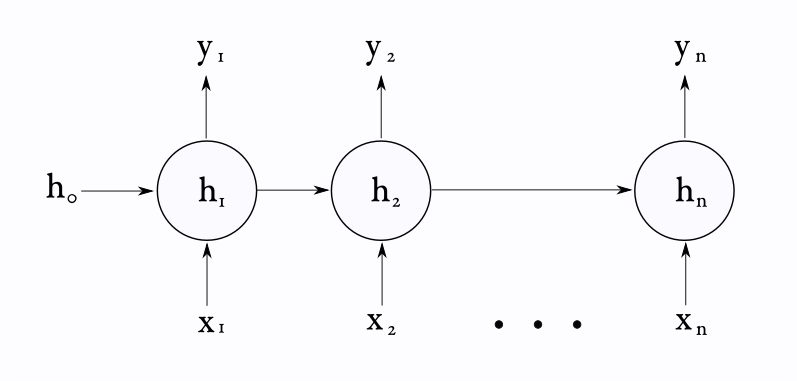
\includegraphics[width=0.5\textwidth]{pics/rnn_network}
  \caption{RNN for NER}
  \label{fig:rnn_network}
\end{figure}
%
At each timestep, the neural network computes a hidden state $ h_t $ using an input 
vector $ x_t $ and the previous hidden state $ h_{t-1} $ that retains information from past 
iterations. Finally, the RNN produces an output vector $ y_t $ representing the label for that 
timestep. A common definition for a RNN cell is given by the equations:
%
\begin{align*}
h_t &= tanh(W_x x_t + W_h h_{t-1}) &\\
y_t &= softmax(W_y h_t) &
\end{align*}
%
Where $ W_x $, $ W_h $ and $ W_y $ are weight matrices that can be trained with the 
Backpropagation Through Time (BPTT) algorithm. Theoretically, RNNs are capable of learning
and retaining long term dependencies through their internal state $ h_t $. However, in practice,
it becomes difficult due to the vanishing gradient problem. Long short term memory networks (LSTM) were 
introduced by Hochreiter and Schmidhuber \cite{Hochreiter1997} with this problem in mind and 
have been popularized since then. 

LSTMs incorporate a memory cell $ c $ in the RNN definition and three gates to control 
the flow of information that comes in and out of the memory cell.
The input gate $ \Gamma_{i} $ controls the amount of new information that will flow into the memory cell,
the forget gate $ \Gamma_{f} $ controls the amount of previous information that will be retained in the memory
cell, and the output gate $ \Gamma_{o} $ controls the amount of information stored in the memory cell that
will be used to compute the output activation of the LSTM unit. 
LSTM cell implementations vary slightly in the literature. A visual description of 
our LSTM cell is provided in Figure~\ref{fig:lstm_cell}.

\begin{figure}[h]
  \centering
  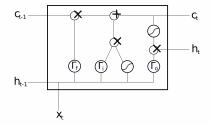
\includegraphics[width=0.5\textwidth]{pics/lstm_cell}
  \caption{LSTM Cell}
  \label{fig:lstm_cell}
\end{figure}

The equations for the LSTM cell are:
%
\begin{align*}
\Gamma_{i} &= \sigma(W_i \cdot [x_t,h_{t-1}] + b_i) &\\
\Gamma_{f} &= \sigma(W_f \cdot [x_t,h_{t-1}] + b_f) &\\ 
\Gamma_{o} &= \sigma(W_o \cdot [x_{t},h_{t-1}] + b_o) &\\
c_t        &= \Gamma_{f} \ast c_{t-1} + \Gamma_{i} \ast tanh(W_c \cdot [x_{t},h_{t-1}] + b_c) &\\
h_t        &= \Gamma_{o} \ast tanh(c_t) &
\end{align*}
%
Where $ \sigma $ is the logistic sigmoid function. $ \Gamma_i $, $ \Gamma_f $, and $ \Gamma_o $ are the input,
forget and output gates, respectively, and $ W_i $, $ W_f $, $ W_o $ are the weight 
matrices corresponding to each gate. $ c_{t} $ is the cell 
state at time $ t $ and $ h_{t} $ is the hidden state at time $ t $. 
The vector $ [x_{t},h_{t-1}] $ is formed by concatenating the current input vector 
$ x_{t} $ and the hidden vector from a previous timestep $ h_{t-1} $. Finally,
$ A \ast B $ represents the element-wise multiplication of matrices $ A $ and $ B $
and $ A \cdot B $ represents the dot product of $ A $ and $ B $.

This implementation differs from the LSTM cell described in Huang et al. \shortcite{Huang2015}
in that the gates $ \Gamma_i $ and $ \Gamma_f $ do not receive inputs from the previous 
cell state $ c_{t-1} $ and the output gate $ \Gamma_{o} $ does not receive inputs from the current cell 
state $ c_{t} $. This variation produces little difference in terms of model accuracy on
the performed task, but it reduces model complexity.

\subsubsection{BI-LSTM-CRF}
\label{sssec:lstm_crf}

On \gls{ner} tasks, both past and future words are important 
to attribute a label at time $ t $, however a regular LSTM network only takes 
past states into consideration. A bidirectional LSTM solves this problem by stacking 
two regular LSTMs, and feeding them with observations in opposite directions. The first LSTM 
receives forward states and the second LSTM receives backward states. The hidden states from both 
networks can then be concatenated at each timestep to produce output labels. With this 
architecture, LSTM cells may use information from past and future timesteps to decide 
the label at time $ t $.

Huang et al. \shortcite{Huang2015} proposed a bidirectional LSTM with a CRF layer (BI-LSTM-CRF) on 
the output to tackle the sequence tagging problem. The main benefit of adding a CRF layer 
in the neural sequence model is that the labels are jointly decoded for a whole sentence 
instead of being predicted individually. 
Predicted tags should be highly correlated 
in a named entity recognition task, so it is desirable to predict sequences conjointly.
The BI-LSTM-CRF is described in Figure~\ref{fig:bi_lstm_crf}.

\begin{figure}[h]
  \centering
  \includegraphics[width=0.5\textwidth]{pics/bi_lstm_crf}
  \caption{Bidirectional LSTM-CRF}
  \label{fig:bi_lstm_crf}
\end{figure}

This architecture achieved a F1 score of 90.10 on the English data from the CoNLL-2003 
NER shared task \cite{KimSang2003}, in contrast to 85.17 for a bidirectional LSTM without 
a CRF layer. 
In our experiments, the LSTM-CRF architecture uses a bidirectional LSTM with 100 
hidden states, no peepholes and input and output dropout layers with a dropout
rate of 0.5. The dropout layers have proven to be very important to prevent overfitting 
and allow better generalization.

\subsubsection{CNN character representations}
\label{sssec:lstm_crf_cnn}

Ma and Hovy \shortcite{Ma2016} proposed to add a convolutional neural network (CNN) layer 
on top of a bidirectional LSTM-CRF to encode character-level information. The CNN
layer is described visually in Figure \ref{fig:cnn}.

\begin{figure}[h]
  \centering
  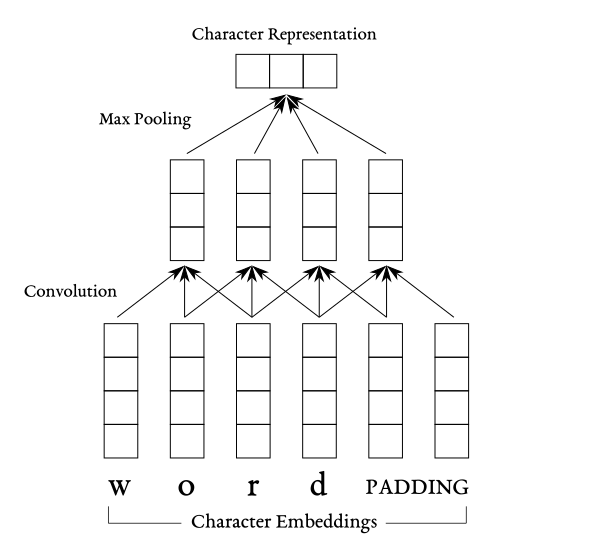
\includegraphics[width=0.5\textwidth]{pics/cnn}
  \caption{CNN based character representations}
  \label{fig:cnn}
\end{figure}

The \gls{cnn} receives character embeddings as inputs and extracts
morphological features by sliding one dimensional filters over the sequence of characters 
and collapsing the filter outputs with a global max pooling layer, producing character
representations with a size determined by the number of filters. 
This means, that when a filter gets a good match at any position in the sequence, the 
max pooling layer output relative to that filter will be triggered, therefore this type of 
character representation detects position invariant morphological features. For example,
the word "finger" would trigger a filter for "ing" the same way the word "writing" would
trigger this filter. The character 
representations generated by the CNN are combined with word level representations 
and fed to the BI-LSTM-CRF described in section \ref{sssec:lstm_crf}.
This architecture can learn morphological features that are very
useful in the NER task, since similar named entities often present morphological similarities. 
This architecture obtained a F1 score of 91.21 in the CoNLL-2003 dataset. In our experiments, 
the LSTM-CRF architecture with CNN character representations uses a one dimensional convolutional 
neural network with 50 filters and a window size of three characters on top of the LSTM-CRF 
architecture. The character embeddings fed to the CNN have 50 dimensions that are randomly 
initialized.

\subsubsection{LSTM character representations}

Lample et al \shortcite{Lample2016} proposed to use a bidirectional LSTM to model character-level 
representations on top of a BI-LSTM-CRF. Combining the forward and backward LSTM hidden states 
to form the character representation, as described in Figure~\ref{fig:lstm_char}. 

\begin{figure}[h]
  \centering
  \includegraphics[width=0.5\textwidth]{pics/lstm_char_representations}
  \caption{LSTM based character representations}
  \label{fig:lstm_char}
\end{figure}

This character representation is also combined with a word 
representation and fed to a BI-LSTM-CRF network. 
The forward state is expected to be a better representation of the suffix of 
a token, and the backward state is expected to be a better representation of 
the prefix of a token. This differentiates the architecture
from the CNN based approach described in Section~\ref{sssec:lstm_crf_cnn}, because CNN filters 
discover positional invariant features, while LSTMs can better represent 
suffixes and prefixes. In our experiments, 
the LSTM-CRF architecture with LSTM character representations was implemented with a bidirectional 
LSTM with 25 hidden states, producing character representations of 
size 50. The character embeddings have 50 dimensions that are randomly initialized.

\subsubsection{Network training}

In the experiments, all neural models were trained using mini batch Stochastic Gradient Descent over 20 epochs with batch size 10,
learning rate 0.001, momentum 0.9 and decay rate 0.05. We used early stopping \cite{Caruana2000} to select the best 
parameters, considering the F1 measure in the validation set. All neural models used 
GloVe 300-dimensional word embeddings \cite{Pennington2014} that were not fine tuned during training.


\section{Researcher Name Extraction Dataset}
\label{cha:dataset}

This section describes the dataset used to evaluate the performance of sequence labeling models
on the \gls{wde} task of \gls{rne}. We call it the \gls{rne} dataset.
We attested experimentally that 
models trained in a popular \gls{ner} dataset (the {CoNLL-2003} English dataset) do not perform 
well in the \gls{rne} task and this is likely due to the differences
between plain text and HTML. The lack of other \gls{ner} 
datasets built for HTML name extraction imposes the need to construct a dataset specific for \gls{rne}.

The \gls{rne} task consists of finding researcher names in faculty listings from university 
webpages across the world, mainly from Computer Science departments.
This would be a necessary step when linking researcher profiles from university 
websites to their entries in public databases. Unlike many
\gls{wde} datasets, each webpage in the \gls{rne} dataset comes from a different 
website, and therefore has a different format, what makes many \gls{wde}
approaches impractical. The idea is to explore systems that are general 
enough to allow accurate entity extraction from different sources while requiring
no supervision between different websites. 

We collected 145 Computer Science and Engineering faculty pages from 42 different countries in
multiple languages, although the English version was preferred when it was available.
We gathered faculty webpages in proportion to
the number of universities in each country\footnote{A detailed list of universities can
be found in https://univ.cc/world.php}. 
University pages that contained 
corrupt HTML or JavaScript code that performed lazy loading of data records were
not included in this dataset.

\subsection{Data Description} 
\label{sec:data_description}

Each of the 145 faculty pages was preprocessed and converted
to the {CoNLL-2003} data format. That is, one word per line with empty lines representing
sentence boundaries. Sentence boundaries were determined by line break HTML tags
(div, p, table, li, br, etc.) in contrast to inline tags (span, em, a, td, etc.). 
Sentences that were more than fifty tokens long were also split according to the
punctuation. Some algorithms have trouble handling very big sentences, so we verified
experimentally that fifty tokens provide a large enough context 
and allow efficient training. 

% The algorithm used for sentence segmentation is described in
% Appendix~\ref{app:html_segmenter}.

A robust tool for HTML segmentation poses many challenges by itself, but the simple approach 
adopted here has proved to be sufficient to perform \gls{rne} adequately. 
Also, it is best to evaluate \gls{ner} models without relying on any sophisticated data 
record segmentation system.
In many cases, entity annotation may precede the segmentation
phase on \gls{wde} methods. Also, depending on the task (as is the case
for researcher name extraction), a good annotator that is able to work 
with raw HTML provides a good solution to the problem.

Finally, all tokens were tagged using the IOB scheme put forward by~\cite{Ramshaw1999}
and used in {CoNLL-2003}, this is:

\begin{quote}
Words tagged with O are outside of named entities
and the I-XXX tag is used for words inside a
named entity of type XXX. Whenever two entities of
type XXX are immediately next to each other, the
first word of the second entity will be tagged B-XXX
in order to show that it starts another entity~\cite{KimSang2003}.
\end{quote}

The \gls{rne} dataset only has entities of type person (PER), therefore a classifier has to
label each token with one of the labels: O, B-PER, or I-PER. 
% This is an example 
% sentence from the dataset:
% 
% \begin{table}[h]
%   \small
%   \begin{center}
%     \begin{tabular}{ ll }
%       Token & Correct Label \\
%       \midrule
%       Kasper    & I-PER \\ 
%       Rasmussen & I-PER \\
%       Associate & O     \\
%       Professor & O     \\    
%       ,         & O     \\    
%       Royal     & O     \\    
%       Society   & O     \\    
%       Research  & O     \\    
%       Fellow    & O     \\    
%     \end{tabular}     
%   \end{center}
% \end{table}
% 
The \gls{rne} dataset was divided in training, validation and test sets, which are described in 
Table~\ref{tab:dataset}. The sizes of the data files were chosen with more or 
less the same proportion adopted in other sequence labeling datasets such
as {CoNLL-2003}, that is described in Table~\ref{tab:conll}. The validation set 
was used in the early stopping 
validation strategy to avoid overfitting classifiers, but model performance 
was only evaluated by comparing the performance in the test set, which is
never observed during training.

\begin{table}[h]
  \small
  \begin{center}
    \begin{tabular}{ lllll }
      \toprule
      Data file & Documents & Sentences & Tokens & Names \\
      \midrule
      Training    & 85  & 24728 & 110269 & 5822  \\  
      Validation  & 30  & 8743  & 36757  & 1788  \\
      Test        & 30  & 10399 & 44795  & 2723  \\
      \midrule
      Total       & 145 & 43870 & 151821 & 10333 \\
      \bottomrule
    \end{tabular}
  \end{center}
  \caption{Description of the data files in the RNE dataset.}
  \label{tab:dataset}
\end{table}

\begin{table}[h]
  \small
  \begin{center}
    \begin{tabular}{ llllllll }
      \toprule
      Data file & Documents & Sentences & Tokens & LOC & MISC & ORG & PER \\
      \midrule
      Training    & 946  & 14987 & 203621 & 7140 & 3438 & 6321 & 6600 \\  
      Validation  & 216  & 3466  & 51362 & 1837 & 922 & 1341 & 1842  \\
      Test        & 231  & 3684  & 46435 & 1668 & 702 & 1661 & 1617  \\
      \midrule
      Total       & 1393 & 22137 & 301418 & 10645 & 5062 & 9323 & 10059 \\
      \bottomrule
    \end{tabular}
  \end{center}
  \caption{Description of the {CoNLL-2003} English dataset}
  \label{tab:conll}
\end{table}


Most webpages in this dataset are faculty directories with informative
text in small passages, however long prose is not absent. 
Size and structure varies wildly, therefore some documents 
may contain up to a few hundred names whereas other documents may contain 
only a dozen names. 

\subsection{Evaluation}
\label{sec:evaluation}

The performance of classifiers in the \gls{rne} dataset was evaluated according to their Precision (P), Recall (R) and F-scores
in the test set. The Precision and Recall 
measures are defined in terms of the number of true positives, false negatives, and false 
positives made by the classifier when extracting named entities. That is:

\begin{equation*}
\text{Precision} = \frac{\text{TruePos}}{\text{TruePos} + \text{FalsePos}}      
\qquad
\text{Recall} = \frac{\text{TruePos}}{\text{TruePos} + \text{FalseNeg}}
\end{equation*}

Precision accounts for the proportion of named entities found by the model that are 
correct relative to all predicted named entities.
Recall is the proportion of named entities correctly predicted by the model relative to
all named entities in the dataset. Precision measures Type I errors 
(false positives) and Recall measures Type II errors (false negatives). Partial matches are
not considered, so a classification only counts as a true positive if the entire named entity
has been correctly extracted. Additionally, the F-score, proposed by~\cite{Rijsbergen1979}, 
is a composite measure that combines Precision and Recall, defined as:

\begin{equation}
F_{\beta} = (1 + \beta^2) \cdot \frac{\text{Precision} \cdot \text{Recall}}{(\beta^2 \cdot \text{Precision}) + \text{Recall}}
\label{eq:fscore_formula}
\end{equation}

The choice of $ \beta $ depends on the relative importance attributed to Precision over Recall.
This formula ``measures the effectiveness of retrieval with respect to a user who attaches 
$ \beta$ times as much importance to recall as precision''~\cite{Rijsbergen1979}. A common choice
for the value of $ \beta $ is $ 1 $, this measure is called the $ F_1 $-score (F1). That is, we attribute 
as much importance to Recall as to Precision.

In our experiments, we considered the Precision, Recall and $ F_1 $-scores over the entire 
data files. Considering that each webpage has a different number of named entities,
this naturally privileges models that work well for pages with more named entities. 
A different approach might be to consider the averaged Precision, Recall and $ F_1 $-scores 
per webpage, privileging systems that have more regularity between different websites. However, 
this approach would cover other deficiencies. That is, the impact of errors in pages with many 
named entities would diminish and the impact of errors in pages with few named entities would
increase. So, the former approach was preferred.


\subsection{Dictionary}
\label{sec:dictionary}

A dictionary of named entities can be a powerful aid to sequence labeling systems,
especially when considering traditional statistical methods. For the \gls{rne} task, we extracted 
a list of 1,595,771 researcher names from the DBLP database and annotated tokens in the
\gls{rne} dataset with exact and partial match tags. That is, if a sequence of tokens
corresponded exactly to a name from the DBLP list, the entire sequence was annotated as 
an exact match. Otherwise, if only some tokens in the sequence matched a name from the DBLP
list partially, the matching tokens were annotated with a partial match tag. This dictionary
was used by some of the models that will be discussed in the experiments section, however it 
must be stated that one of the main advantages of Deep Neural Networks relative to other
approaches is the fact that they can perform well even without the aid of a dictionary.

\begin{table}[h]
  \small
  \begin{center}
    \begin{tabular}{ lllll }
      \toprule
      Data file & Precision & Recall & F1 & Correct names \\
      \midrule
      Training   & 0.7316 & 0.2303 & 0.3504 & 1341 of 5822 \\ 
      Validation & 0.8474 & 0.2858 & 0.4274 & 511 of 1788 \\ 
      Test       & 0.8717 & 0.3268 & 0.4754 & 890 of 2723 \\ 
      \bottomrule
    \end{tabular}
  \end{center}
  \caption{DBLP dictionary coverage in each data file of the RNE dataset.}
  \label{tab:gazetteer}
\end{table}

To understand how this dictionary can be useful for some models in the \gls{rne}, 
we consider the Precision, Recall and $ F_1 $-scores for an exact dictionary matching 
strategy in each \gls{rne} data file. The results are described in 
Table~\ref{tab:gazetteer}. These results also provide a baseline with which to compare
other methods of sequence labeling. 
The reported performance was obtained by only extracting named entities that corresponded to an exact 
match. Any useful extraction method should at least improve upon this approach.
Recall is very low because the dictionary is incomplete and Precision falls short of
top performing extraction methods. This last result is surprising since we are only extracting 
exact matches. The reason for the low Precision is that exact dictionary matches may actually 
only correspond to partial matches in the dataset. For example, if the dictionary has an entry
for "Ann Smith", it may partially overlap an entry in the dataset for "Mary Ann Smith", yielding
a false positive.


\subsection{Comparison with {CoNLL-2003}}
\label{sec:conll_comparison}

The {CoNLL-2003} dataset introduced in the \gls{ner}
shared-task in 2003 is frequently used to attest 
the performance of state-of-the-art sequence labeling systems~\cite{Huang2015,Lample2016,Ma2016,Peters2018}. 
The English data is composed of news stories extracted from the Reuters Corpus, and 
provides annotations for four types of entities: people (PER), organizations (ORG), 
locations (LOC), and miscellaneous (MISC), which includes entities that cannot be 
classified in one of the former groups. The statistics for the {CoNLL-2003} dataset 
were already described in Table~\ref{tab:conll}.

Considering this dataset, it comes to mind why exactly do we need a \gls{ner} dataset for HTML. 
If the {CoNLL-2003} English dataset is used to both train and evaluate 
state-of-the-art models, it is to be expected that models trained in this dataset will
be able to extract the same named entities in other documents with reasonable 
effectiveness. However, this is hardly the case. By intuition, we know that tabular HTML 
documents, such as faculty listings, are very different from plain text. But with the
RNE dataset for \gls{ner} on HTML, we can understand how different they really are.

We trained three classifiers to perform the task of person name extraction using
the {CoNLL-2003} training set. The {CoNLL-2003} dataset was relabeled so that classifiers only had to extract
person entities (PER labels), thus other entity types (LOC, ORG, and MISC) were relabeled as
not an entity (O label). We trained the classifiers with the relabeled {CoNLL-2003} training set,
and validated the results with the relabeled validation set. The models were tested with the relabeled {CoNLL-2003}
test set and the \gls{rne} test set.
In Table~\ref{tab:conll_to_ner_on_html}, we present the results for a first order \gls{hmm}, 
a Linear Chain \gls{crf}, and a Bi-LSTM-CRF classifier with GloVe embeddings~\cite{Huang2015} in the 
aforementioned experimental setting.

\begin{table}[h]
  \small
  \begin{center}
    \begin{tabular}{ lllllll }
      \toprule
      \multirow{2}{*}{Model} & \multicolumn{3}{c}{CoNLL-2003} & \multicolumn{3}{c}{\gls{rne}} \\
                             & \multicolumn{1}{c}{P} & \multicolumn{1}{c}{R} & \multicolumn{1}{c}{F1}
                             & \multicolumn{1}{c}{P} & \multicolumn{1}{c}{R} & \multicolumn{1}{c}{F1} \\
      \midrule
      HMM         & 0.777 & 0.452 & 0.571 & 0.189 & 0.180 & 0.184 \\
      CRF         & 0.774 & 0.754 & 0.764 & 0.138 & 0.129 & 0.133 \\
      Bi-LSTM-CRF & 0.969 & 0.931 & 0.950 & 0.282 & 0.258 & 0.269 \\
      \bottomrule
    \end{tabular}
  \end{center}
  \caption{
    Performance of three classifiers trained with the {CoNLL-2003} training set and tested in
    the CoNLL-2003 and RNE test sets.
  }
  \label{tab:conll_to_ner_on_html}
\end{table}

The very low $ F_1 $-score obtained by all models in the \gls{rne} test set is worse than the established
dictionary baseline. We cannot use these results to properly compare the relative performances 
between the models (this topic will be explored in the next section), but it is possible to conclude
that machine learning models trained in plain text do not necessarily perform very well in HTML 
extraction tasks. The Bi-LSTM-CRF model obtained a 0.269 $ F_1 $-score in the \gls{rne} test
set, what is surprising considering that it is a very efficient approach to sequence labeling in plain 
text. By looking at some of its mistakes we can shed some light on this result. The Bi-LSTM-CRF model
extracted "Dean Emeritus" and "14101 INF" as names, and it missed the last names in "George E. Elliott"
and "Carl J. Galligan". These mistakes are representative of some of the major flaws with the systems
trained with the CoNLL-2003 training set. The names in the \gls{rne} dataset 
are usually longer than in CoNLL-2003 and the word distributions are vastly different, what may
account for some of the mistakes of the Bi-LSTM-CRF model.

Lets consider some other differences between both datasets. 
The number of documents in the \gls{rne} dataset is much smaller: only 145 against 
1393. However, the number of sentences in the \gls{rne}
dataset is higher: 43870 against 22137. Also, the number of tokens in the \gls{rne} dataset
is roughly half the number present in the {CoNLL-2003} dataset. These numbers show that 
the HTML documents in the \gls{rne} dataset are longer than news 
stories and, more importantly, they are composed of much shorter sentences when compared 
to the text from news corpora (3.46 words per sentence in the \gls{rne} dataset
against 13.62 words per sentence in {CoNLL-2003}). Most faculty webpages have a lot of 
boilerplate text that contributes to their size, while the news stories in {CoNLL-2003}
are usually rather short. These numbers show that HTML provides far less context to be made 
use by sequence models, what imposes the need to seek other sources of evidence in addition to 
the text, such as dictionaries and the HTML structure.

Another aspect that differs among the NER datasets is the word distributions. Word frequencies
tend to vary considerably in documents with different topics. Table~\ref{tab:frequent_words}
shows the ten most frequent words for each dataset, including punctuation signs. Punctuation
signs are frequently present in proper names, as in: Mary B. Smith, Susan (Susie) Williams, John Al-Azzawi, etc.
Also, punctuation signs can be useful to detect boundaries between named entities.
The {CoNLL-2003} English dataset contains a more generic selection of terms whereas the 
subject of the \gls{rne} dataset becomes evident with words such as "professor" and "university" 
happening with a high frequency in the corpus. Also, punctuation signs are much more frequent in
the \gls{rne} dataset. 

Lastly, in Figure~\ref{fig:word_frequency_plot}
we plot the word frequencies for the hundred most frequent words in the {CoNLL-2003} and 
the \gls{rne} datasets. In both plots we have a few very frequent words and a long tail of
infrequent words. In the \gls{rne} dataset, most named entities are located in this long tail, 
therefore a good sequence labeling method needs to be able to handle the labeling of infrequent 
tokens effectively. 
Table~\ref{tab:unknown_tokens} shows the number of unknown tokens~\footnote{
Unknown tokens are tokens that occur at least once in the validation or test sets 
but do not occur in the training set.
}
in the validation and test
sets of the \gls{rne} dataset, and the number of named entities that contain at least one 
unknown token. Roughly four in every five named entities contain at least one unknown
token.

\begin{table}[h]
  \small
  \begin{center}
    \begin{tabular}{ llll }
      \toprule
      \multicolumn{2}{c}{CoNLL-2003} & \multicolumn{2}{c}{\gls{rne}} \\
      \multicolumn{1}{c}{Word} & \multicolumn{1}{c}{Frequency} &
      \multicolumn{1}{c}{Word} & \multicolumn{1}{c}{Frequency} \\
      \midrule
      the & 12310 & , & 10439      \\
      , & 10876 & - & 8140         \\
      . & 10874 & ) & 3655         \\
      of & 5502 & ( & 3641         \\
      in & 5405 & : & 3484         \\
      to & 5129 & of & 3345        \\
      a & 4731 & and & 2499        \\
      ( & 4226 & professor & 2456  \\
      ) & 4225 & university & 1611 \\
      and & 4223 & research & 1315 \\
      \bottomrule
    \end{tabular}
  \end{center}
  \caption{Ten most frequent words for the {CoNLL-2003} dataset and the RNE dataset.}
  \label{tab:frequent_words}
\end{table}

\begin{table}[h]
  \small
  \begin{center}
    \begin{tabular}{ lllll }
      \toprule
      Tokens / Named Entities (NE) & Valid & \% & Test & \%\\
      \midrule
      Unknown Tokens & 12076 & 26.96\% & 8324  & 22.65\% \\
      Known Tokens   & 32719 & 73.04\% & 28433 & 77.35\% \\
      Total          & 44795 & 100.00\%   & 36757 & 100.00\%   \\
      \midrule
      NEs with Unknown Tokens    & 1446 & 80.87\% & 2205 & 80.98\% \\
      NEs without Unknown Tokens & 342  & 19.13\% & 518  & 19.02\% \\
      Total                      & 1788 & 100.00\% & 2723 & 100.00\%   \\
      \bottomrule
    \end{tabular}
  \end{center}
  \caption{Unknown tokens in the RNE dataset.}
  \label{tab:unknown_tokens}
\end{table}

\begin{figure}[h!]
  \begin{center}
    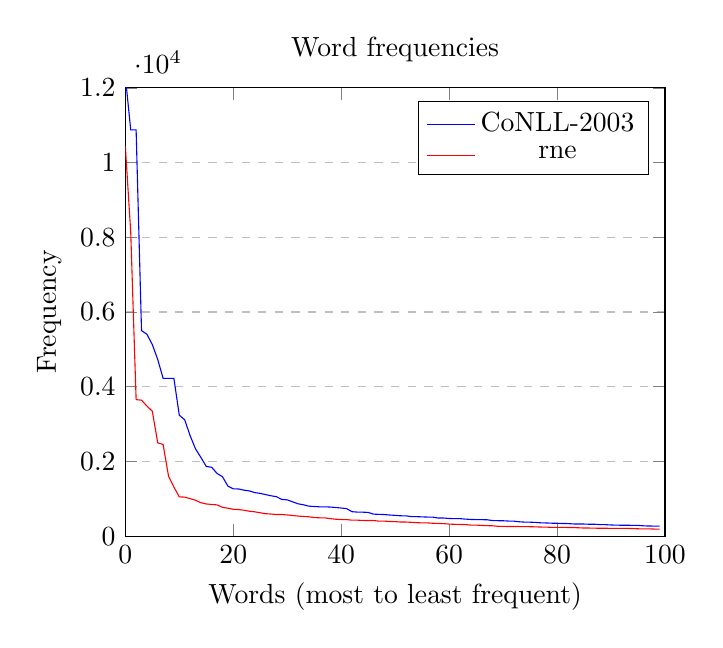
\begin{tikzpicture}
      \begin{axis}[
        title={Word frequencies},
        xmin=0, xmax=100,
        ymin=0, ymax=12000,
        ylabel={Frequency},
        xlabel={Words (most to least frequent)},
        ymajorgrids=true,
        grid style=dashed,
        legend pos=north east,
        % scaled y ticks=false,
      ]

      \addplot[color=blue, color=blue] coordinates {
        (0,12310)(1,10876)(2,10874)(3,5502)(4,5405)(5,5129)(6,4731)(7,4226)(8,4225)(9,4223)(10,3239)(11,3115)(12,2694)(13,2339)(14,2109)(15,1866)(16,1845)(17,1679)(18,1593)(19,1342)(20,1267)(21,1264)(22,1232)(23,1212)(24,1166)(25,1146)(26,1113)(27,1082)(28,1057)(29,984)(30,973)(31,920)(32,867)(33,841)(34,804)(35,796)(36,786)(37,786)(38,780)(39,768)(40,754)(41,738)(42,656)(43,645)(44,643)(45,636)(46,591)(47,584)(48,579)(49,567)(50,558)(51,546)(52,545)(53,524)(54,523)(55,517)(56,512)(57,510)(58,486)(59,486)(60,474)(61,470)(62,470)(63,457)(64,448)(65,444)(66,442)(67,441)(68,419)(69,415)(70,413)(71,405)(72,402)(73,386)(74,377)(75,375)(76,369)(77,358)(78,354)(79,348)(80,346)(81,340)(82,338)(83,328)(84,327)(85,325)(86,320)(87,319)(88,310)(89,308)(90,300)(91,296)(92,293)(93,292)(94,291)(95,289)(96,278)(97,272)(98,271)(99,271)
      };
      \addplot[color=red, color=red] coordinates {
        (0,10439)(1,8140)(2,3655)(3,3641)(4,3484)(5,3345)(6,2499)(7,2456)(8,1611)(9,1315)(10,1053)(11,1046)(12,1006)(13,963)(14,897)(15,863)(16,849)(17,838)(18,773)(19,749)(20,720)(21,713)(22,695)(23,668)(24,652)(25,626)(26,602)(27,593)(28,581)(29,580)(30,569)(31,553)(32,539)(33,527)(34,520)(35,499)(36,492)(37,490)(38,469)(39,454)(40,446)(41,444)(42,429)(43,429)(44,422)(45,420)(46,419)(47,403)(48,403)(49,394)(50,390)(51,379)(52,379)(53,371)(54,362)(55,356)(56,355)(57,346)(58,342)(59,337)(60,324)(61,318)(62,314)(63,311)(64,298)(65,297)(66,288)(67,282)(68,279)(69,265)(70,263)(71,259)(72,259)(73,258)(74,258)(75,254)(76,250)(77,245)(78,243)(79,236)(80,236)(81,235)(82,234)(83,232)(84,225)(85,219)(86,218)(87,215)(88,212)(89,212)(90,210)(91,209)(92,208)(93,208)(94,205)(95,198)(96,197)(97,196)(98,191)(99,191)
      };
      \legend{CoNLL-2003, \gls{rne}};
       
      \end{axis}
    \end{tikzpicture}
    \caption{
      Word frequencies plot for the {CoNLL-2003} dataset and the RNE dataset.
    }
    \label{fig:word_frequency_plot}
  \end{center}
\end{figure}


\section{Experiments}

The main objective of this article is to compare the best methods for \gls{ner} on the 
web considering the \gls{rne} task. The value of a specific method is determined
not only by its accuracy, but also by the amount of feature engineering required, the training
time required, and the overall complexity of the model when we consider its gains relative to
simpler alternatives. All models were trained on Amazon G3.4xlarge instances, which are equipped with 
NVIDIA Tesla M60 GPUs with 8GB internal memory, however all the HMM operations were done in the CPU.
The implementations were done entirely in Python using Google's Tensorflow deep learning 
library~\footnote{https://www.tensorflow.org/.}. 
Subsection~\ref{ssec:exp_1} discusses the results of featureless models and Subsection~\ref{ssec:exp_2} 
discusses models that incorporated features and a dictionary.


\subsection{Featureless models}
\label{ssec:exp_1}

The first experiment aimed to evaluate the performance of sequence models that used 
only words as features in the \gls{rne} task.
A model that works well despite the absence of a good feature selection is arguably more valuable than
a method that requires feature engineering or a big dictionary of named entities, as long as 
its accuracy is sufficiently high for the intended purpose. This is where Deep Neural Networks are most
useful. However, the improved accuracy of neural architectures comes at the expense of more complexity
and a longer training time, what must also be taken into account. 
The tested HMMs and CRFs used only the unaccented lowercase version of the current token as a feature
to predict labels at each timestep. The neural networks used GloVe-300 word embeddings using the 
unaltered token as a lookup index. Due to the rugged shape of the loss function, the neural networks 
do not necessarily converge to an optimal set of parameters, so the reported results are the averages
over five runs of each model. 

Table \ref{tab:experiment1} shows the Precision (P), Recall (R), F1-scores (F1) and the time to 
train the models and run predictions (Time) for HMMs up to third order, CRFs, and Bi-LSTM-CRFs with
CNN-based character representations (CNNc) and LSTM-based character representations (LSTMc).

\begin{table}[h]
  \small
  \begin{center}
    \begin{tabular}{ llllllll }
      \toprule
      \multirow{2}{*}{Model} & \multicolumn{3}{c}{Validation} & \multicolumn{3}{c}{Test} & \multirow{2}{*}{Time} \\
                             & \multicolumn{1}{c}{P} & \multicolumn{1}{c}{R} & \multicolumn{1}{c}{F1}
                             & \multicolumn{1}{c}{P} & \multicolumn{1}{c}{R} & \multicolumn{1}{c}{F1} & \\
      \midrule
      HMM-1                 & 0.693 & 0.581 & 63.2 & 0.637 & 0.458 & 53.3 & 15.72   \\
      HMM-2                 & 0.703 & 0.630 & 66.5 & 0.653 & 0.527 & 58.3 & 31.32   \\
      HMM-3                 & 0.616 & 0.618 & 61.7 & 0.551 & 0.468 & 50.6 & 80.69   \\
      CRF                   & 0.806 & 0.805 & 80.6 & 0.795 & 0.710 & 75.0 & 918.25  \\
      Bi-LSTM-CRF           & 0.906 & 0.938 & 92.2 & 0.909 & 0.865 & 88.6 & 2580.30 \\
      Bi-LSTM-CRF+CNNc      & 0.929 & 0.946 & 93.8 & \textbf{0.921} & 0.881 & 90.1 & 3379.33 \\
      Bi-LSTM-CRF+LSTMc     & 0.928 & 0.950 & 93.9 & 0.920 & \textbf{0.886} & \textbf{90.2} & 4412.41 \\
      \bottomrule
    \end{tabular}
  \end{center}
  \caption{Precision, recall and F1 in the RNE dataset for models that incorporate no features}
  \label{tab:experiment1}
\end{table}

Without resorting to features besides the current word or a dictionary of named entities, HMMs and CRFs have a
poor performance. Increasing the number of previous timesteps considered by the HMM helps
up to a point, but its effectiveness is limited. The second order HMM (HMM-2) achieves a 58.3 F1
while the third order HMM (HMM-3) suffers a drop in performance with a 50.6 F1. The CRF is the
best classical model, achieving a 75.0 F1 in the test set.

All neural models achieved a considerably better performance in the RNE task. The plain Bi-LSTM-CRF
achieved a 88.6 F1. Character representations improved the performance by a little amount,
to 90.1 F1 for the CNN-based representations and to 90.2 F1 for the LSTM-based
representations. In CoNLL-2003, the reported results were 91.2 F1 for the CNN-based
representations~\cite{Ma2016} and 90.9 F1 for the LSTM-based representations~\cite{Lample2016}, improving
upon the plain Bi-LSTM-CRF model~\cite{Huang2015}, which achieved a 90.1 F1. These results seem to be in
accord with our own experiments for the \gls{rne} dataset, with the primary difference that the
LSTM-based character representations were more effective in our experimental setting,
contrasting with the CoNLL-2003 results.
Nevertheless, the difference between the two types of character representations 
is not substantial enough to allow a solid conclusion about the quality of
one model over the other. However, the benefit of adding character representations 
to plain recurrent neural networks is clearly supported by the evidence.


\subsection{All features}
\label{ssec:exp_2}

Eleven discrete features were extracted from the dataset. 
These were selected from a larger pool of features, 
considering their aid to the performance of the extraction systems. Deep learning 
architectures can work incredibly well without any of these features, however they
are of critical importance to traditional approaches such as HMMs and CRFs. 
The selected features are presented in Table~\ref{tab:features}. 

\begin{table}[h]
  \small
  \begin{center}
    \begin{tabular}{ lll }
      \toprule
      Feature & Description & Type \\
      \midrule
      1  & Unaccented lowercase token & Categorical \\
      2  & Exact dictionary match & Binary \\
      3  & Partial dictionary match & Binary \\
      4  & Is an Email & Binary \\
      5  & Contains a Number & Binary \\
      6  & Is an Honorific (Mr., Mrs., Dr., etc.) & Binary \\
      7  & Is a URL & Binary \\
      8  & Is capitalized & Binary \\
      9  & Is a punctuation sign & Binary \\
      10 & HTML tag + parent & Categorical \\
      11 & CSS class & Categorical \\
      \bottomrule
    \end{tabular}
  \end{center}
  \caption{Features used in the RNE dataset.}
  \label{tab:features}
\end{table}

Features 2 and 3 relate to the dictionary extracted from DBLP described in Section~\ref{cha:dataset}.
Feature 10 is the token's enclosing HTML tag and its parent tag concatenated.
Feature 11 is the CSS class for the token's HTML tag.
Features 10 and 11 are only useful in the self-training strategy for HMMs, because
the patterns represented by these features are webpage specific. In other models, we only used
features 1 to 9.

Table \ref{tab:experiment2} shows the results for the models that incorporated features. 
The self trained HMMs are described with the suffix +ST.

\begin{table}[h]
  \small
  \begin{center}
    \begin{tabular}{ llllllll }
      \toprule
      \multirow{2}{*}{Model} & \multicolumn{3}{c}{Validation} & \multicolumn{3}{c}{Test}                       & \multirow{2}{*}{Time} \\
                             & \multicolumn{1}{c}{P}          & \multicolumn{1}{c}{R} & \multicolumn{1}{c}{F1}
                             & \multicolumn{1}{c}{P}          & \multicolumn{1}{c}{R} & \multicolumn{1}{c}{F1} & \\
      \midrule
      HMM-1                & 0.730 & 0.714 & 72.2 & 0.826 & 0.684 & 74.8 & 15.22 \\
      HMM-2                & 0.720 & 0.710 & 71.5 & 0.820 & 0.724 & 76.9 & 30.10 \\
      HMM-3                & 0.721 & 0.702 & 71.1 & 0.791 & 0.667 & 72.4 & 81.14 \\
      HMM-1+ST             & 0.747 & 0.906 & 81.9 & 0.866 & 0.867 & 86.6 & 28.54 \\
      HMM-2+ST             & 0.771 & 0.912 & 83.5 & 0.885 & 0.869 & 87.7 & 57.52 \\
      HMM-3+ST             & 0.788 & 0.917 & 84.7 & 0.826 & 0.803 & 81.4 & 154.67 \\
      CRF                  & 0.881 & 0.903 & 89.2 & 0.870 & 0.786 & 82.6 & 965.59 \\
      Bi-LSTM-CRF          & 0.918 & 0.947 & 93.2 & 0.926 & 0.878 & 90.1 & 2261.79 \\
      Bi-LSTM-CRF+CNNc     & 0.918 & 0.956 & 93.7 & \textbf{0.933} & \textbf{0.902} & \textbf{91.7} & 3255.93 \\
      Bi-LSTM-CRF+LSTMc    & 0.904 & 0.958 & 93.0 & 0.912 & 0.875 & 89.3 & 4249.21 \\
      \bottomrule
    \end{tabular}
  \end{center}
  \caption{Precision, recall and F1 in the RNE dataset for models that incorporate all features}
  \label{tab:experiment2}
\end{table}

Conventional models like HMMs, and CRFs can become quite competitive with
the right selection of features and a good gazetteer, however they still have worse F1 scores
than the neural models without features, demonstrating their inherent limitations.
Second-order HMMs (HMM-2) performed consistently better than
the other HMM variants. The self-training strategy was effective in improving the 
performance of all HMMs considerably. The best model (HMM-2) went from a 76.9 F1 to
87.7 F1, with a substantial improvement in Recall (0.724 to 0.869). As with the 
featureless models, the CRF is superior to the HMMs that did not incorporate the self-training
strategy, achieving 82.6 F1.

The inclusion of features in the neural models had no decisive positive effect. The plain 
Bi-LSTM-CRF and the model with CNN-based character representations had an increase in 
F1, 90.1 and 91.7 respectively, but the Bi-LSTM-CRF with LSTM-based character representations 
actually suffered a slight decrease in performance relative to the featureless model. 
Overall, the power of deep neural networks for sequence labeling lies 
in their remarkable capacity to perform well without resorting to features besides the raw text. 
The small difference in performance between featureless neural networks and neural networks 
with features demonstrates that the CNN or LSTM character representations seem to be effective 
in extracting morphological features automatically and the pre-trained GloVe word embeddings 
can outweigh the absence of a gazetteer, since named entities that belong to the same category
tend to have similar embeddings.

Despite the superior performance of Neural Networks in this task, there remains an important 
consideration to be made. As we increase the complexity and the training time required by the models, there 
is only a scant gain in terms of F1. For example, the 
Bi-LSTM-CRF with LSTM character representations achieved a 90.2 F1, while 
the HMM-2 using a Self-Training strategy achieved a 87.9 F1. It is a small difference
in performance, considering the disparity of model complexity. This reality
is not limited to the RNE dataset. For example, 
the winning NER model in the CoNLL-2003 competition~\cite{Florian2003} used a combination of simple
statistical models and feature engineering to achieve 88.76 F1 in the English test set, 
while the Bi-LSTM-CRF with LSTM characters achieved 90.94 F1~\cite{Lample2016} and the Bi-LSTM-CRF with 
CNN characters achieved 91.21 F1~\cite{Ma2016}. That is,
the improvement is below three points in the F1 score.

The Neural Network approach to NER does not demand any feature engineering or self-training, 
contrasting with the HMM approach, which is highly reliant on
the right selection of features and the self-training strategy. However, the absence of
human intervention in Deep Neural Networks is questionable to some degree since there is the
need to define many hyper parameters and
details about the neural architecture, such as the number of \textit{LSTM} layers and
hidden weights, where to add dropout layers, which pre-trained word embeddings to use, etc. In summary, 
there are many choices to be made, none of which have definitive theoretical justification, 
so the model variations need to be tested empirically. This requires many iterations between setting
parameters, obtaining results, and tuning parameters once again. Considering that each of 
these iterations can take at least a couple of hours to finish, it is not clear if
selecting features is necessarily a more arduous struggle.

To the best of our abilities, the Tensorflow implementation of the Bi-LSTM-CRF + LSTMc
model running on a AWS GPU instance took approximately 4412 seconds to train 
and run predictions. While, the HMM-2 did the same in approximately
58 seconds, running in a conventional CPU with unoptimized code. This is almost 80 times 
faster, what is relevant if we are trying to improve the models over many iterations.
Finally, if we consider the intellectual cost of understanding and implementing both 
models and the code maintainability of both implementations, the difference becomes even 
more profound.


\section{Conclusion}

Machine-learning-based sequence labeling models are an effective approach for NER 
both on plain text and on web data extraction tasks. 
In this article, we compared the performance of HMMs, CRFs and Neural Networks on the task of
researcher name extraction, introducing a novel dataset that is publicly available,
the RNE dataset.
Models trained in plain text are not effective to perform NER on the web, because 
HTML pages contain a substantial amount of boilerplate text and the sentences are shorter 
than typical plain text, what confounds the classifiers. The results for the RNE dataset
confirm many results reported in the natural language processing literature, but it also 
demonstrates that different web extraction tasks will most likely demand specific labeled 
datasets. 

Constructing labeled datasets for sequence labeling is awfully expensive, especially if we
are interested in extracting more than a couple of entity types. This leads to the
conclusion that unsupervised or at least semi-supervised extraction methods are a more 
prosperous line of research. Unfortunately, the performance of unsupervised systems is still
not comparable to what can be achieved with supervised systems.

The neural architectures for sequence labeling performed better than other models in the 
researcher name extraction task. Among them, the Bi-LSTM-CRF with LSTM-based character 
representations achieved a 90.2 F1 in the task using only GloVe-300 word embeddings. By adding
textual features and a gazetteer, the Bi-LSTM-CRF with CNN-based character representations
achieved a 91.7 F1 in the test set of the RNE dataset. However, these neural architectures are
quite complex, demanding sophisticated decisions such as the choice of hyper parameters for the 
optimization method, the number of LSTM layers, where to add dropout layers, and the choice of 
word embeddings. All of these decisions
must be tested empirically since there is seldom theoretical justification for one choice over
the other.

In contrast to deep neural networks, the Hidden Markov Model is a very simple approach to 
sequence labeling that can provide a satisfactory solution to NER on the web. In the researcher
name extraction task, the second-order HMM using a good selection of features and the self-training
strategy achieved a 87.7 F1, taking only 57 seconds to train and run predictions, while neural 
network models took between 40 and 80 times longer to do the same with more expensive hardware.
Depending on the end goal, this should be taken in consideration. However, neural models are
undeniably more accurate and more flexible.

The effective recognition of named entities on HTML is an essential step in most general 
\gls{wde} methods. The accuracy achieved by deep neural architectures
shows the potential for a truly flexible approach to cross domain extraction.
Also, the self-training strategy showed a remarkable effectiveness in boosting the performance 
of all HMM variants. It did so by using knowledge about the HTML context to make predictions,
inspired on classical \gls{wde} systems. Future work could incorporate this 
knowledge on neural models or CRFs to boost their performance in web extraction
tasks.


% \bibliographystyle{named}
% \bibliography{bibfile}

% \begin{thebibliography}{}
%   \bibitem[\protect\citename{Akmajian and Lehrer }1976]{akm76}
%   Akmajian, A. and Lehrer, A. (1976) NP-like quantifiers and the
%   problem of determining the head of an NP. {\it Linguistic
%   Analysis\/} {\bf 2}: 295--313.
%   \bibitem[\protect\citename{Huddleston }1984]{hud84}
%   Huddleston, Rodney. (1984) {\it Introduction to the Grammar of
%   English}. Cambridge: Cambridge University Press.
%   \bibitem[\protect\citename{McCord }1990]{mcc90}
%   McCord, Michael C. (1990) Slot grammar: a system for simpler
%   construction of practical natural language grammars. In R.
%   Studer (ed.), {\it Natural Language and Logic: International
%   Scientific Symposium}, pp.~118--45. Lecture Notes in Computer
%   Science. Berlin: Springer-Verlag.
%   \bibitem[\protect\citename{Salton {\it et al.}\ }1990]{sal90}
%   Salton, Gerald, Zhao, Zhongnan and Buckley, Chris. (1990)
%   A simple syntactic approach for the generation of indexing
%   phrases. Technical Report 90--1137, Department of Computer
%   Science, Cornell University.
% \end{thebibliography}

\bibliographystyle{apa}

\begin{thebibliography}{}

\bibitem[\protect\citename{Abdessalem T., Cautis B., and Derouiche N. }{2010}]{Abdessalem2010}
Abdessalem T., Cautis B., and Derouiche N. (2010)
ObjectRunner: Lightweight, targeted extraction and querying of structured web data.
In {\it Proceedings of the VLDB Endowment}
{\bf 3(1-2)}: 1585--1588.

\bibitem[\protect\citename{Adelberg }1998]{Adelberg1998}
Adelberg B. (1998)
NoDoSE---a tool for semi-automatically extracting structured and semistructured data from text documents.
{\it ACM SIGMOD Record} 
{\bf 27(2)}: 283--294.

\bibitem[\protect\citename{Akbik, Blythe and Vollgraf }2018]{Akbik2018}
Akbik, A., Blythe, D. and Vollgraf, R. (2018)
Contextual string embeddings for sequence labeling.
In {\it Proceedings of the 27th International Conference on Computational Linguistics}
pp. 1638--1649, Santa Fe, New Mexico, ACL.

\bibitem[\protect\citename{Arocena and Mendelzon }1998]{Arocena1999}
Arocena, G. and Mendelzon, A. (1998)
WebOQL: Restructuring documents, databases, and webs.
In {\it Proceedings of the Fourteenth International Conference on Data Engineering (ICDE '98)}
pp. 24--33, Washington, DC, USA, IEEE Computer Society.

\bibitem[\protect\citename{Baevski, Edunov, Liu, Zettlemoyer and Auli }2019]{Baevski2019}
Baevski, A., Edunov, S., Liu, Y., Zettlemoyer, L. and Auli, M. (2019)
Cloze-driven pretraining of self-attention networks.
{\it Preprint arXiv:1903.07785}.

\bibitem[\protect\citename{Bikel, Schwartz and Weischedel }1999]{Bikel1999}
Bikel, D., Schwartz, R. and Weischedel, R. (1999)
An algorithm that learns what's in a name.
{\it Machine Learning}
{\bf 34(1)}: 211--231.

\bibitem[\protect\citename{Borthwick, Sterling, Agichtein and Grishman }1998]{Borthwick1998}
Borthwick, A., Sterling, J., Agichtein, E. and Grishman, R. (1998)
Exploiting diverse knowledge sources via maximum entropy in named entity recognition.
In {\it Proceedings of the Sixth Workshop on Very Large Corpora}
pp. 152--160. ACL.

\bibitem[\protect\citename{Califf and Mooney }1999]{Califf1999}
Califf, M. and Mooney, R. (1999)
Relational learning of pattern-match rules for information extraction.
{\it Computational Linguistics}
{\bf 4}: 9--15.

\bibitem[\protect\citename{Caruana, Lawrence and Giles }2000]{Caruana2000}
Caruana, R., Lawrence, S. and Giles, L. (2000)
Overfitting in neural nets: Backpropagation, conjugate gradient, and early stopping.
In {\it Proceedings of the 13th International Conference on Neural Information Processing Systems (NIPS'00)}
pp. 381--387, Cambridge, MA, USA, MIT Press.

\bibitem[\protect\citename{Chang and Lui }2001]{Chang2001}
Chang, C. and Lui, S. (2001)
IEPAD: information extraction based on pattern discovery.
In {\it Proceedings of the 10th international conference on World Wide Web}
pp. 681--688.

\bibitem[\protect\citename{Chang and Kuo }2004]{Chang2004}
Chang, C. and Kuo, S. (2004)
OLERA: Semisupervised Web-data extraction with visual support.
{\it IEEE Intelligent Systems}
{\bf 19(6)}: 56--64.

\bibitem[\protect\citename{Chang, Kayed, Girgis and Shaalan }2006]{Chang2006}
Chang, C., Kayed, M., Girgis, M. and Shaalan, K. (2006)
A Survey of Web Information Extraction Systems.
{\it IEEE Transactions on Knowledge and Data Engineering}
{\bf 18(10)}: 1411--1428.

\bibitem[\protect\citename{Collobert, Weston, Bottou, Karlen, Kavukcuoglu, and Kuksa }2011]{Collobert2011}
Collobert, R., Weston, J., Bottou, L., Karlen, M., Kavukcuoglu, K. and Kuksa P. (2011)
Natural language processing (almost) from scratch.
{\it Journal of Machine Learning Research}
{\bf 12}: 2493--2537.

\bibitem[\protect\citename{Crescenzi, Mecca, and Merialdo }2001]{Crescenzi2001}
Crescenzi V., Mecca G., and Merialdo P. (2001)
Roadrunner: Towards automatic data extraction from large web sites.
In {\it Proceedings of the 27th International Conference on Very Large Data Bases}, 
pp. 109--118.

\bibitem[\protect\citename{Devlin, Chang, Lee, and Toutanova }2018]{Devlin2018}
Devlin, J., Chang, M., Lee, K. and Toutanova, K. (2018)
{BERT}: Pre-training of deep bidirectional transformers for language understanding.
{\it Preprint arXiv:1810.04805}.

\bibitem[\protect\citename{Dong, Gabrilovich, Heitz, Horn, Lao, Murphy, Strohmann, Sun, and Zhang }{2014}]{Dong2014}
Dong, X., Gabrilovich, E., Heitz, G., Horn, W., Lao, N., Murphy, K., Strohmann, T., Sun, S. and Zhang, W. (2014)
Knowledge Vault: a web-scale approach to probabilistic knowledge fusion.
In {\it Proceedings of the 20th ACM SIGKDD international conference on Knowledge discovery and data mining (KDD '14)}
pp. 601--610.

\bibitem[\protect\citename{Ferrara and Baumgartner }2011]{Ferrara2011}
Ferrara, E. and Baumgartner, R. (2011)
Automatic wrapper adaptation by tree edit distance matching.
{\it Smart Innovation, Systems and Technologies}
{\bf 8}: 41--54.

\bibitem[\protect\citename{Ferrara, De Meo, Fiumara and Baumgartner }2014]{Ferrara2014}
Ferrara, E., De Meo, P., Fiumara, G. and Baumgartner, R. (2014)
Web data extraction, applications and techniques: A survey.
{\it Knowledge-Based Systems}
{\bf 70}: 301--323.

\bibitem[\protect\citename{Florian, Ittycheriah, Jing and Zhang }2003]{Florian2003}
Florian, R. Ittycheriah, A. Jing, H. and Zhang, T. (2003)
Named entity recognition through classifier combination.
In {\it Proceedings of the Seventh Conference on Natural Language Learning at HLT-NAACL 2003}
pp. 168--171.

\bibitem[\protect\citename{Freitag }1998]{Freitag1998}
Freitag, D. (1998)
Information Extraction from HTML: Application of a General Machine Learning Approach.
In {\it Proceedings of the Fifteenth National/Tenth Conference on Artificial Intelligence/Innovative Applications of Artificial Intelligence (AAAI '98/IAAI '98)}
pp. 517--523, Menlo Park, CA, USA, American Association for Artificial Intelligence.

\bibitem[\protect\citename{Freitag and Mccallum }1999]{Freitag1999}
Freitag, D. and Mccallum, A. (1999)
Information Extraction with HMMs and Shrinkage.
In {\it Proceedings of the AAAI-99 Workshop on Machine Learning for Information Extraction}
pp. 31--36. AAAI Press.

\bibitem[\protect\citename{Freitag and McCallum }2000]{Freitag2000}
Freitag, D. and McCallum, A. (2000)
Information Extraction with HMM Structures Learned by Stochastic Optimization.
In {\it Proceedings of the Seventeenth National Conference on Artificial Intelligence and Twelfth Conference on Innovative Applications of Artificial Intelligence}
pp. 584--589. AAAI Press.

\bibitem[\protect\citename{Furche, Gottlob, Grasso, Gunes, Guo, Kravchenko, Orsi, Schallhart, Sellers, and Wang }{2012}]{Furche2012}
Furche, T., Gottlob, G., Grasso, G., Gunes, O., Guo, X., Kravchenko, A., Orsi, G., Schallhart, C., Sellers, A., and Wang, C. (2012)
Diadem: Domain-centric, intelligent, automated data extraction methodology.
In {\it Proceedings of the 21st International Conference on World Wide Web (WWW '12 Companion)}, 
pp. 267--270, New York, ACM.

\bibitem[\protect\citename{Hammer, McHugh and Garcia-Molin }1997]{Hammer1997}
Hammer, J., McHugh, J. and Garcia-Molin, H. (1997)
Semistructured Data: The TSIMMIS Experience.
In {\it Proceedings of the First East-European Conference on Advances in Databases and Information Systems (ADBIS'97)}
pp. 22--22, Swindon, UK, BCS Learning \& Development Ltd.

\bibitem[\protect\citename{Hsu and Dung }{1998}]{Hsu1998}
Hsu, Chun-Nan and Dung Ming-Tzung. (1998) 
Generating finite-state transducers for semi-structured data extraction from the Web.
{\it Information Systems \/}, 
{\bf 23(8)}: 521--538.

\bibitem[\protect\citename{Laender, Ribeiro-Neto, da Silva }2002a]{Laender2002a}
Laender, A., Ribeiro-Neto, B. and da Silva, A. (2002)
DEByE - Date extraction by example.
{\it Data Knowledge Engineering}
{\bf 40(2)}: 121--154.

\bibitem[\protect\citename{Laender, Ribeiro-Neto, da Silva and Teixeira }2002b]{Laender2002b}
Laender, A., Ribeiro-Neto, B., da Silva, A., and Teixeira, J. (2002)
A brief survey of web data extraction tools.
{\it SIGMOD Record}
{\bf 31(2)}: 84--93.

\bibitem[\protect\citename{Liu, Pu and Han }2000]{Liu2000}
Liu, L., Pu, C. and Han, W. (2000)
XWRAP: an XML-enabled wrapper construction system for Web information sources.
In {\it Proceedings of 16th International Conference on Data Engineering}
pp. 611--621.

\bibitem[\protect\citename{Hochreiter and Schmidhuber }1997]{Hochreiter1997}
Hochreiter, S. and Schmidhuber, J. (1997)
Long short-term memory.
{\it Neural Computation}
{\bf 9(8)}: 1735--1780.

\bibitem[\protect\citename{Hogue and Karger }2005]{Hogue2005}
Hogue, A. and Karger, D. (2005)
Thresher: Automating the Unwrapping of Semantic Content from the World Wide Web.
In {\it Proceedings of the 14th International Conference on World Wide Web (WWW '05)}
pp. 86--95, New York, NY, USA, ACM.

\bibitem[\protect\citename{Huang, Xu and Yu }2015]{Huang2015}
Huang, Z., Xu, W. and Yu, K. (2015)
Bidirectional {LSTM-CRF} models for sequence tagging.
{\it CoRR}, abs/1508.01991.

\bibitem[\protect\citename{Kim~Sang and De-Meulder }2003]{KimSang2003}
Kim-Sang, T. and De~Meulder, F. (2003)
Introduction to the CoNLL-2003 Shared Task: Language-independent Named Entity Recognition.
In {\it Proceedings of the Seventh Conference on Natural Language Learning at HLT-NAACL 2003 - Volume 4 (CONLL '03)}
pp. 142--147, Stroudsburg, PA, USA, ACL.

\bibitem[\protect\citename{Krupl, Herzog and Gatterbauer }2005]{Krupl2005}
Krupl, B. Herzog, M. and Gatterbauer, W. (2005)
Using visual cues for extraction of tabular data from arbitrary HTML documents.
{\it Special interest tracks and posters of the 14th international conference on World Wide Web - WWW '05} 
pp. 1000--1001.

\bibitem[\protect\citename{Kushmerick }2000]{Kushmerick2000}
Kushmerick, N. (2000) 
Wrapper induction: efficiency and expressiveness.
{\it Artificial Intelligence\/} 
{\bf 118(1-2)}: 15--68.

\bibitem[\protect\citename{Lafferty, McCallum and Pereira }2001]{Lafferty2001}
Lafferty, J., McCallum, A. and Pereira, F. (2001)
Conditional random fields: Probabilistic models for segmenting and labeling sequence data.
In {\it Proceedings of the Eighteenth International Conference on Machine Learning (ICML '01)}, 
pp. 282--289, San Francisco, CA, USA, Morgan Kaufmann Publishers Inc.

\bibitem[\protect\citename{Lample, Ballesteros, Subramanian, Kawakami and Dyer }2016]{Lample2016}
Lample, G., Ballesteros, M., Subramanian, S., Kawakami, K. and Dyer, C. (2016)
Neural architectures for named entity recognition.
{\it CoRR}, abs/1603.01360.

\bibitem[\protect\citename{Li and Gray }2000]{Li2000}
Li, J. and Gray, R. (2000)
Image Segmentation and Compression Using Hidden Markov Models.
Kluwer Academic Publishers, Norwell, MA, USA.

\bibitem[\protect\citename{Liu and Nocedal }1989]{Liu1989}
Liu, D. and Nocedal, J. (1989)
On the limited memory bfgs method for large scale optimization.
{\it Mathematical Programming}
{\bf 45(1)}: 503--528.

\bibitem[\protect\citename{Ma and Hovy }2016]{Ma2016}
Ma, X. and Hovy, E. (2016)
End-to-end sequence labeling via bi-directional {LSTM}-{CNN}s-{CRF}.
In {\it Proceedings of the 54th Annual Meeting of the Association for Computational Linguistics (Volume 1: Long Papers)}
pp. 1064--1074, Berlin, Germany, ACL.

\bibitem[\protect\citename{McCallum, Freitag and Pereira }2000]{McCallum2000}
McCallum, A., Freitag, D. and Pereira, F. (2000)
Maximum entropy markov models for information extraction and segmentation.
In {\it Proceedings of the Seventeenth International Conference on Machine Learning (ICML '00)}
pp. 591--598, San Francisco, CA, USA, Morgan Kaufmann Publishers Inc.

\bibitem[\protect\citename{McCallum and Li }2003]{McCallum2003}
McCallum, A. and Li, W. (2003)
Early results for named entity recognition with conditional random fields, feature induction and web-enhanced lexicons.
In {\it Proceedings of the Seventh Conference on Natural Language Learning at HLT-NAACL 2003 - Volume 4 (CONLL '03)}
pp. 188--191, Stroudsburg, PA, USA, ACL.

\bibitem[\protect\citename{Muslea, Minton and Knoblock }1999]{Muslea1999}
Muslea I., Minton S., and Knoblock C. (1999) 
A Hierarchical Approach to Wrapper Induction.
In {\it Proceedings of the Third Annual Conference on Autonomous Agents}, 
pp.~190--197, New York: ACM.

\bibitem[\protect\citename{Pennington, Socher and Manning }2014]{Pennington2014}
Pennington, J., Socher, R. and Manning, C. (2014)
Glove: Global vectors for word representation.
In {\it Empirical Methods in Natural Language Processing (EMNLP)}
pp. 1532--1543.

\bibitem[\protect\citename{Peters, Neumann, Iyyer, Gardner, Clark, Lee and Zettlemoyer }2018]{Peters2018}
Peters, M., Neumann, M., Iyyer, M., Gardner, M., Clark, C., Lee, K. and Zettlemoyer, L. (2018)
Deep contextualized word representations.
In {\it Proceedings of the 2018 Conference of the North American Chapter of the Association for Computational Linguistics: Human Language Technologies, Volume 1 (Long Papers)}
pp. 2227--2237, New Orleans, Louisiana, ACL.

\bibitem[\protect\citename{Rabiner }1990]{Rabiner1990}
Rabiner, L. (1990)
Readings in Speech Recognition. Chapter: A Tutorial on Hidden Markov Models and Selected Applications in Speech Recognition.
Morgan Kaufmann Publishers Inc., San Francisco, CA, USA.

\bibitem[\protect\citename{Ramshaw and Marcus }1999]{Ramshaw1999}
Ramshaw, L. and Marcus, M. (1999)
Text Chunking Using Transformation-Based Learning, 
pp. 157--176. Springer Netherlands, Dordrecht, 1999.

\bibitem[\protect\citename{Ratnaparkhi }1998]{Ratnaparkhi1998}
Ratnaparkhi, A. (1998)
Maximum Entropy Models for Natural Language Ambiguity Resolution.
{\it PhD thesis}, Philadelphia, PA, USA.

\bibitem[\protect\citename{Ribas, Ribeiro-Neto, de Souza e Silva, Ueda, and Ziviani }2015]{Ribas2015}
Ribas, S., Ribeiro-Neto, B., de Souza e Silva, E., Ueda, A., and Ziviani, N. (2015)
In {\it Proceedings of the 24th International Conference on World Wide Web (WWW '15 Companion)}, 
pp. 603--608, New York, ACM.

\bibitem[\protect\citename{Rijsbergen }1979]{Rijsbergen1979}
Rijsbergen, C. (1979)
Information Retrieval.
Butterworth-Heinemann, Newton, MA, USA, 2nd edition.

\bibitem[\protect\citename{Sahuguet and Azavant }1999]{Sahuguet1999}
Sahuguet, A. and Azavant F. (1999)
Building Light-Weight Wrappers for Legacy Web Data-Sources Using W4F.
In {\it Proceedings of the 25th International Conference on Very Large Data Bases (VLDB '99)}
pp. 738--741, San Francisco, CA, USA, Morgan Kaufmann Publishers Inc.

\bibitem[\protect\citename{Sarawagi }2008]{Sarawagi2008}
Sarawagi, S. (2008)
Information extraction.
{\it Foundations and Trends in Databases}
{\bf 1(3)}: 261--377.

\bibitem[\protect\citename{Schulz, Lassig and Gaedke }2016]{Schulz2016}
Schulz, A. Lassig, J. and Gaedke, M. (2016)
Practical web data extraction: Are we there yet? --- A short survey.
{\it IEEE/WIC/ACM International Conference on Web Intelligence (WI), 2016}, 
pp. 562--567.

\bibitem[\protect\citename{Shi, Liu, Shen, Yuan and Huang }{2015}]{Shi2015}
Shi, S., Liu, C., Shen, Y., Yuan, C. and Huang, Y. (2015)
AutoRM: An effective approach for automatic Web data record mining.
{\it Knowledge-Based Systems}
{\bf 89}: 314--331.

\bibitem[\protect\citename{Soderland }1999]{Soderland1999}
Soderland, S. (1999)
Learning Information Extraction Rules for Semi-Structured and Free Text.
{\it Machine Learning} 
{\bf 34(1)}: 233--272.

\bibitem[\protect\citename{Sundheim }1991]{Sundheim1991}
Sundheim. B. (1991)
Overview of the third message understanding evaluation and conference.
In {\it Proceedings of the 3rd Conference on Message Understanding (MUC3 '91)}
pp. 3--16, Stroudsburg, PA, USA, ACL.

\bibitem[\protect\citename{Varlamov and Turdakov }2016]{Varlamov2016}
Varlamov, M. and Turdakov, D. (2016)
A survey of methods for the extraction of information from Web resources.
{\it Programming and Computer Software}
{\bf 42(5)}: 279--291.

\bibitem[\protect\citename{Zhu, Nie, Wen, Zhang, and Ma }2005]{Zhu2005}
Zhu J., Nie Z., Wen J., Zhang B., and Ma W. (2005)
2D Conditional Random Fields for Web Information Extraction.
In {\it Proceedings of the 22Nd International Conference on Machine Learning (ICML '05)}, 
pp.~1044--1051, New York: ACM.

\bibitem[\protect\citename{Zhu, Nie, Wen, Zhang, and Ma }2006]{Zhu2006}
Zhu J., Nie Z., Wen J., Zhang B., and Ma W. (2006)
Simultaneous Record Detection and Attribute Labeling in Web Data Extraction.
In {\it Proceedings of the 12th ACM SIGKDD International Conference on Knowledge Discovery and Data Mining (KDD '06)}, 
pp.~494--503, New York: ACM.

\end{thebibliography}
\end{document}
